\documentclass[12pt]{article}

\usepackage{amssymb}
\usepackage{amsmath}
\usepackage{graphicx}
\usepackage{comment}
\usepackage{textcomp}
\usepackage{xcolor}

\usepackage{natbib}

\setlength{\parindent}{0pt}
\usepackage[margin=3cm]{geometry}

%\renewcommand{\myvecf}{\underline{\mathbf{f}}}
\newcommand{\myvec}[1]{\underline{\mathbf{#1}}}

%\begin{document}
%\documentclass{article}
%\usepackage[utf8]{inputenc}
%\usepackage{amsmath}

%\title{FEM Example}
%\author{apr }
%\date{May 2018}

%\usepackage{graphicx}


\setlength{\parindent}{0mm}% Removes the indents.
\begin{document}

\begin{center}
{\Huge   MECH3750 PBL Content Summary}

\vspace{6mm}

{\Huge  Week 11}

\end{center}

\vspace{6mm}

{\Large Content:}
{\begin{itemize}
	\item Elliptic PDEs
	\begin{itemize}
		\item[--] Numerical Solution
		\item[--] Grid Generation
	\end{itemize}
\end{itemize}}

\vspace{4mm}

{\Large Upcoming assessment:}
{\begin{itemize}
	\item Problem Sheet 11 (due before Week 12 PBL session)
	\item Assignment II (Due tomorrow)
\end{itemize}}

\vspace{4mm}

{Tutors: Nathan Di Vaira, Alex Muirhead, William Snell, Tristan Samson, Nicholas Maurer, Jakob Ivanhoe, Robert Watt}

%{Tutors: Nathan Di Vaira, Alex Muirhead, William Snell, Tristan Samson, Nicholas Maurer, Jakob Ivanhoe, Robert Watt}

\pagebreak

\section{Elliptic PDEs}

The final type of PDE we look at in this course are elliptic PDEs. The most simple example of an elliptic PDE is Laplace's equation,

\vspace{2mm}

\begin{align*}
\frac{\partial^2u}{\partial x^2} + \frac{\partial^2u}{\partial y^2} &= 0  \\[0.8em]
\nabla^2u &= 0 \\[0.8em]
\Delta u &= 0
\end{align*}

\vspace{4mm}

The case when there is a source term (i.e., the PDE is non-homogenous) is known as Poisson's equation.

\vspace{4mm}

Elliptic PDEs have no time derivative, and hence typically solve steady state systems (temperature distributions and potential fields). The solution is therefore influenced only by boundary conditions, not initial conditions. As with other PDEs, types of boundary value problems may include Dirichlet, Neumann or mixed boundaries.

\subsection{Numerical Solution}

To solve elliptic PDEs numerically, we take a centred finite difference approximation for each spatial derivative,

\vspace{2mm}

$$ \frac{u_{i-1,j} - 2u_{i,j} + u_{i+1,j}}{(\Delta x)^2} + \frac{u_{i,j-1} - 2u_{i,j} + u_{i,j+1}}{(\Delta y)^2} = 0,$$

\vspace{4mm}

which now deals with two discrete dimensions, $i$ and $j$. This can be rearrange to give the general update equation for inner nodes,

\vspace{2mm}

$$ u_{i,j} = \frac{(\Delta y)^2 (u_{i-1,j}+u_{i+1,j}) + (\Delta x)^2 (u_{i,j-1}+u_{i,j+1})}{2((\Delta x)^2 + (\Delta y)^2)}. $$

\vspace{4mm}

While the solution nodes are in two-dimensions, the solution vector must be assembled as a single-ordinate vector. The rows of the matrix are assembled by moving along each row of nodes. Detailed examples with code were given in the lecture for how to efficiently handle this.

\vspace{4mm}

Due to the large size of the solution matrix, iterative methods, such as Gauss-Seidel, may be required to solve...

\subsection{Application to Grid Generation}

It turns out that elliptic PDEs are particularly useful for handling complex computational grids. The general idea is that we treat the complex {\it physical} grid, such as a curve, as a {\it computational} square grid.

\begin{figure}[h!]
\centering
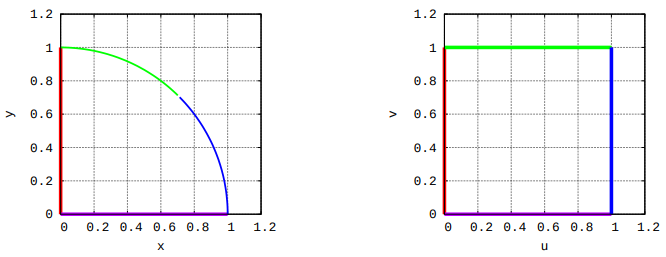
\includegraphics[scale=0.55]{figures/grid_generation_elliptic.png}
\end{figure}

The edge points in the $x$-$y$ domain become the boundary conditions in the $u$-$v$ domain, and we then solve for $x$ and $y$ using two different eliptic equations, 

\vspace{2mm}

\begin{align*}
\frac{\partial^2x}{\partial u^2} + \frac{\partial^2x}{\partial v^2} &= 0  \\[0.8em]
\frac{\partial^2y}{\partial u^2} + \frac{\partial^2y}{\partial v^2} &= 0
\end{align*}

\vspace{4mm}

where $x$ and $y$ are the variables being solved for in each.

\vspace{4mm}

The example attached to the {\it W11L03} lecture gives an excellent example of how this is implemented.

\subsection{Other Considerations}

When handling Neumann boundaries, a simple approach is to use a one-sided finite difference approximation,

\vspace{2mm}

$$ \frac{\partial u}{\partial x} \approx \frac{u_{N,j} - u_{N-1,j}}{\Delta x}. $$

\vspace{4mm}

Additionally, using the central difference approximations shown above for interior nodes give a second order global spatial order of accuracy. Note that boundary approximations of one order less than the interior approximations generally do not reduce the global second order accuracy.


\end{document}
